\section{RESULTADOS}\label{cap:resultsANDdiscussion}

\subsection{Estructura de los Resultados}\label{sec:results}

This chapter presents the results of the research and provides an interpretation of their implications for heart rate classification in infants. The chapter is divided into two main sections: Results and Discussion.

\subsection{Resultados: Estudio 1}\label{sec:resultados-estudio-1}

\subsubsection{Frecuencia Cardiaca}

\begin{table}[H]
    \centering
    \begin{tabular}{|c|c|c|c|}
        \hline
        \textbf{Media Horaria} & \textbf{p-valor} & \textbf{p-valor 
        cuantiles} & \textbf{p-valor 
        escalada} \\
        \hline
        MEAN\_1 & 0.129 & 0.142 & 0.902 \\
        MEAN\_2 & 0.254 & 0.412 & 0.825 \\
        MEAN\_3 & 0.143 & 0.105 & 0.925 \\
        MEAN\_4 & 0.331 & 0.309 & 0.867 \\
        MEAN\_5 & 0.077 & 0.042 & 0.355 \\
        MEAN\_6 & 0.098 & 0.1 & 0.5 \\
        MEAN\_7 & 0.357 & 0.232 & 0.474 \\
        MEAN\_8 & 0.182 & 0.218 & 0.975 \\
        MEAN\_9 & 0.158 & 0.241 & 0.83 \\
        MEAN\_10 & 0.316 & 0.423 & 0.211 \\
        MEAN\_11 & 0.609 & 0.637 & 0.045 \\
        MEAN\_12 & 0.035 & 0.005 & 0.382 \\
        MEAN\_13 & 0.293 & 0.144 & 0.603 \\
        MEAN\_14 & 0.169 & 0.17 & 0.727 \\
        MEAN\_15 & 0.214 & 0.335 & 0.722 \\
        MEAN\_16 & 0.094 & 0.136 & 0.652 \\
        MEAN\_17 & 0.127 & 0.132 & 0.943 \\
        MEAN\_18 & 0.476 & 0.816 & 0.56 \\
        MEAN\_19 & 0.128 & 0.086 & 0.731 \\
        MEAN\_20 & 0.2 & 0.186 & 0.947 \\
        MEAN\_21 & 0.391 & 0.592 & 0.643 \\
        MEAN\_22 & 0.157 & 0.198 & 0.875 \\
        MEAN\_23 & 0.1 & 0.026 & 0.445 \\
        MEAN\_24 & 0.204 & 0.187 & 0.95 \\
        \hline
    \end{tabular}\label{tab:mean-FC}
    \caption{p-valor de la media horaria de la \textit{Frecuencia Cardiaca} y la \textit{Frecuencia Cardiaca Transformada por Cuantiles} entre pacientes que sufren OAF y los que no}
\end{table}

De manera gráfica el resultado es el siguiente mostrado en la Figura~\ref{fig:mean-FC}. Se han añadido dos rectas verticales que muestran el nivel del valor $\alpha$ = 0.05 y $\alpha$ = 0.001. Se puede observar que la mayoría de las medias horarias no son significativas, por lo que no se puede rechazar la hipótesis nula. Esto significa que no hay diferencias significativas entre las medias horarias de la \textit{Frecuencia Cardíaca} entre pacientes que sufren DETERIORO y los que no.

Se puede observar como de manera general que a los pacientes que se les suministra OAF tienen una mayor \textit{Frecuencia Cardíaca} que los que no. Esto se puede observar en la Figura~\ref{fig:fc-boxplot-mean}, aun así no se puede afirmar que esto tenga un efecto significativo de manera general en toda la monitorización del paciente.

Las medias más significativas son las referentes a las horas 12 y 23. Esta situación va a causar a la hora de realizar el \textit{Estudio 2} se tendrán problemas a la hora de realizar un modelo de clasificación dónde los valores de monitorización de la \textit{Frecuencia Cardíaca} sean significativos a la hora de clasificar pacientes como DETERIORO o no.

\begin{figure}[H]
    \centering
    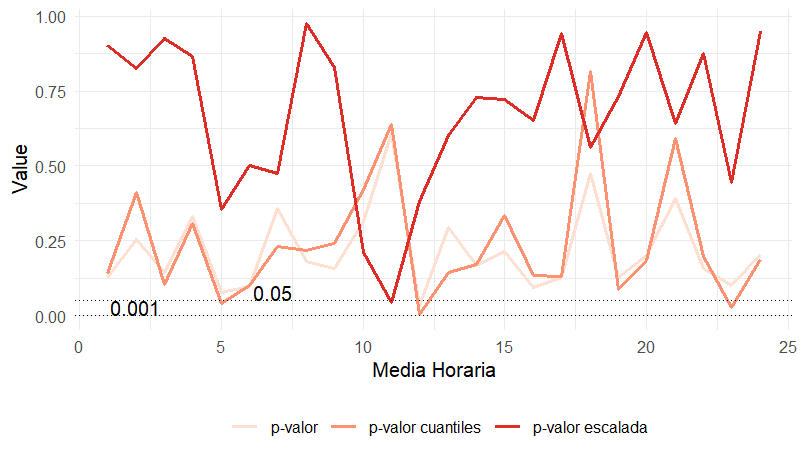
\includegraphics[scale = 1]{./img/mean-FC.png}
    \caption{p-valor de la media horaria de la \textit{Frecuencia Cardiaca} entre pacientes que sufren DETERIORO y los que no}
    \label{fig:mean-FC}
\end{figure}

\newpage
\thispagestyle{empty}
% Se modifica la geometría (los márgenes) de la página y se coloca en formato horizontal:
\newgeometry{top=10mm, bottom=10mm, left=12mm, right=12mm}
\begin{landscape}
\begin{figure}[H]
    \centering
    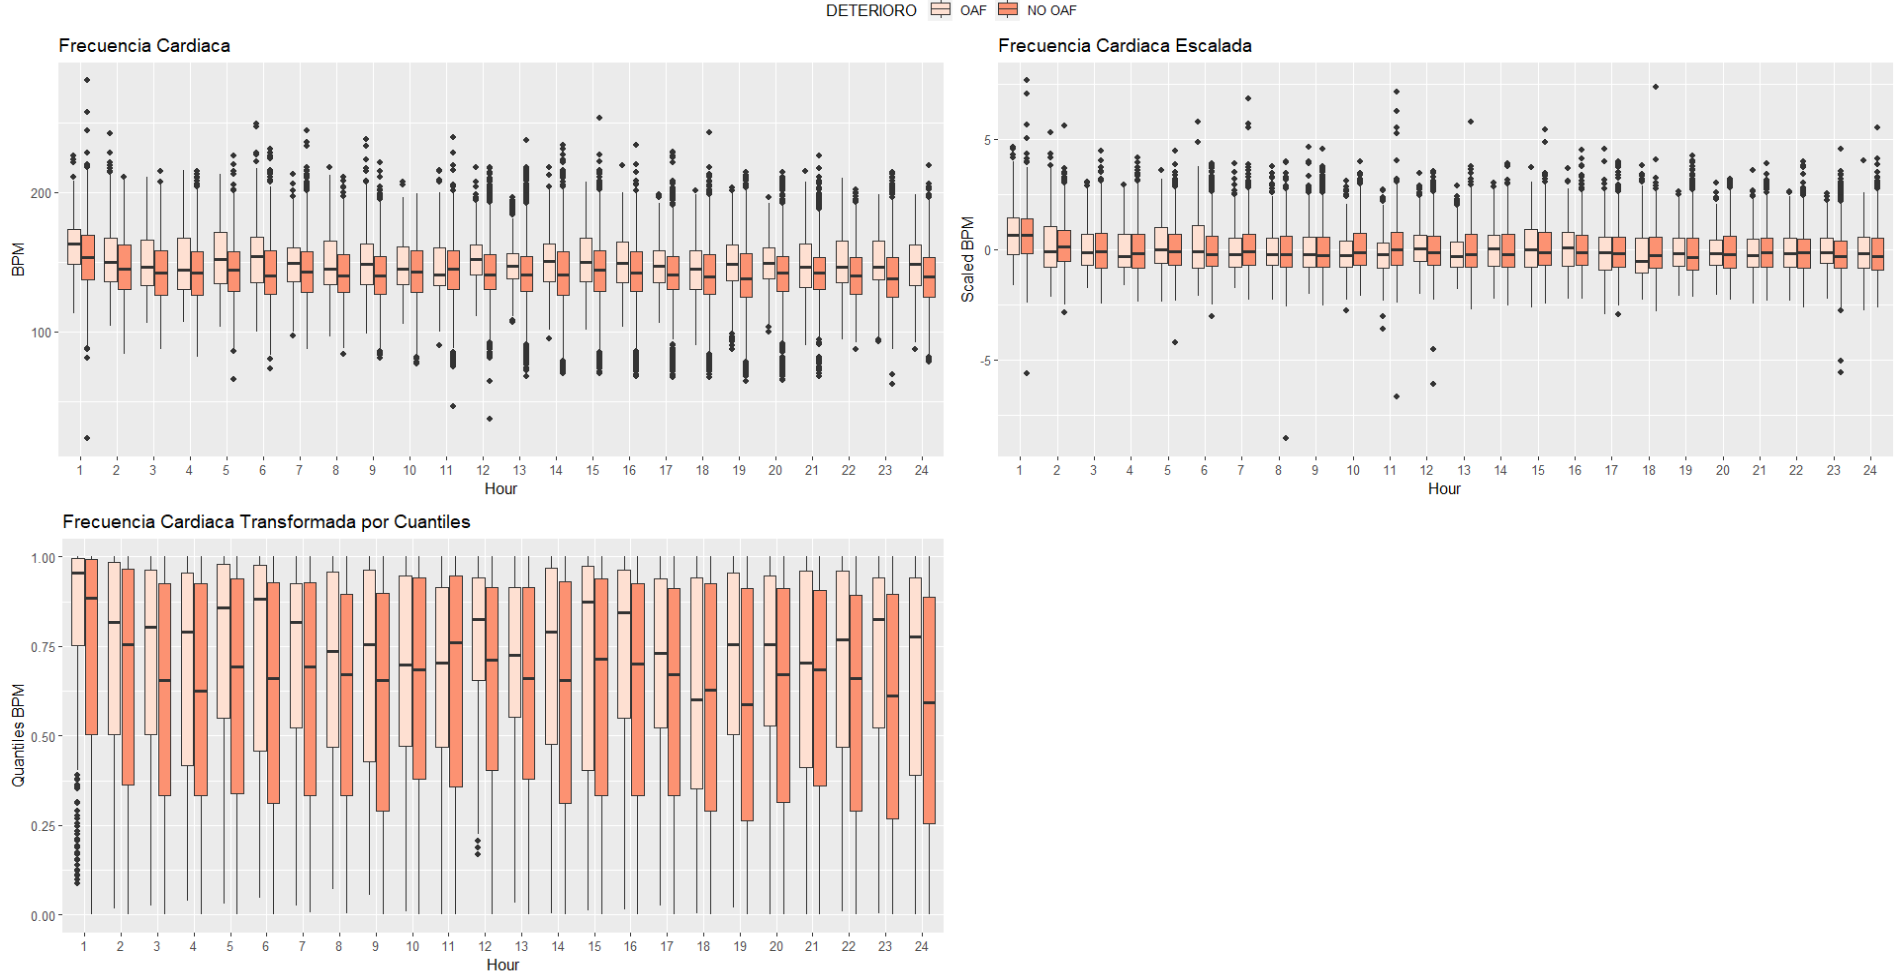
\includegraphics[scale = 0.68]{./img/fc-boxplot-mean.png}
    \caption{Media Horaria de la \textit{Frecuencia Cardíaca}, \textit{Frecuencia Cardíaca Escalada} y la \textit{Frecuencia Cardíaca Transformada por Cuantiles} entre pacientes que sufren DETERIORO y los que no}
    \label{fig:fc-boxplot-mean}
\end{figure}
\end{landscape}
\restoregeometry

\subsubsection{Saturación de Oxígeno}

\begin{table}[H]
    \centering
    \begin{tabular}{|c|c|c|}
        \hline
        \textbf{Media Horaria} & \textbf{p-valor} & \textbf{p-valor escalada} \\
        \hline
        MEAN\_1 & 0.151 & 0.176 \\
        MEAN\_2 & 0.015 & 0.017 \\
        MEAN\_3 & 0.52 & 0.778 \\
        MEAN\_4 & 0.343 & 0.608 \\
        MEAN\_5 & 0.349 & 0.718 \\
        MEAN\_6 & 0.672 & 0.639 \\
        MEAN\_7 & 0.141 & 0.078 \\
        MEAN\_8 & 0.868 & 0.769 \\
        MEAN\_9 & 0.571 & 0.939 \\
        MEAN\_10 & 0.549 & 0.842 \\
        MEAN\_11 & 0.991 & 0.643 \\
        MEAN\_12 & 0.44 & 0.581 \\
        MEAN\_13 & 0.312 & 0.427 \\
        MEAN\_14 & 0.968 & 0.797 \\
        MEAN\_15 & 0.641 & 0.966 \\
        MEAN\_16 & 0.799 & 0.183 \\
        MEAN\_17 & 0.312 & 0.993 \\
        MEAN\_18 & 0.89 & 0.204 \\
        MEAN\_19 & 0.543 & 0.71 \\
        MEAN\_20 & 0.384 & 0.784 \\
        MEAN\_21 & 0.867 & 0.503 \\
        MEAN\_22 & 0.665 & 0.195 \\
        MEAN\_23 & 0.882 & 0.294 \\
        MEAN\_24 & 0.889 & 0.358 \\
        \hline
    \end{tabular}
    \caption{p-valor de la media horaria de la \textit{Saturación de O$_2$} entre pacientes que sufren OAF y los que no}
\end{table}

Al igual que en el apartado anterior el resultado es el siguiente mostrado en la Figura~\ref{fig:mean-SatO2}. La mayoría de las medias horarias no son significativas, por lo que no se puede rechazar la hipótesis nula. Esto significa que no hay diferencias significativas entre las medias horarias de la \textit{Saturación de O$_2$} entre pacientes que sufren DETERIORO y los que no.

Se puede observar como de manera general que a los pacientes que se les suministra OAF tienen una mayor \textit{Saturación de O$_2$} que los que no. Esto se puede observar en la Figura~\ref{fig:satO2-boxplot-mean}, aun así no se puede afirmar que esto tenga un efecto significativo de manera general en toda la monitorización del paciente.

La única media significativa menor que $\alpha = 0.05$ es la monitorizada en la hora $2$ .Al igual que en el apartado anterior, esta situación va a causar a la hora de realizar el \textit{Estudio 2} se tendrán problemas a la hora de realizar un modelo de clasificación dónde los valores de monitorización de la \textit{Saturación de O$_2$} sean significativos a la hora de clasificar pacientes como DETERIORO o no.



\begin{figure}[H]
    \centering
    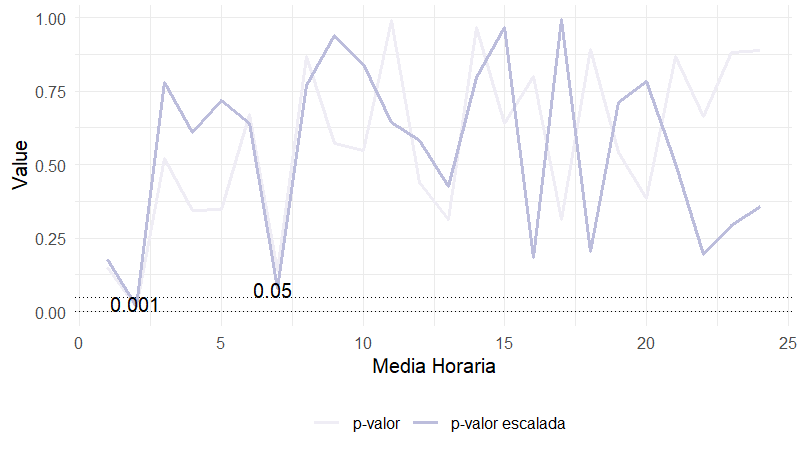
\includegraphics[scale = 1]{./img/mean-SatO2.png}
    \caption{p-valor de la media horaria de la \textit{Saturación de Oxígeno} entre pacientes que sufren DETERIORO y los que no}
    \label{fig:mean-SatO2}
\end{figure}

\newpage
\thispagestyle{empty}
% Se modifica la geometría (los márgenes) de la página y se coloca en formato horizontal:
\newgeometry{top=10mm, bottom=10mm, left=12mm, right=12mm}
\begin{landscape}
\begin{figure}[H]
    \centering
    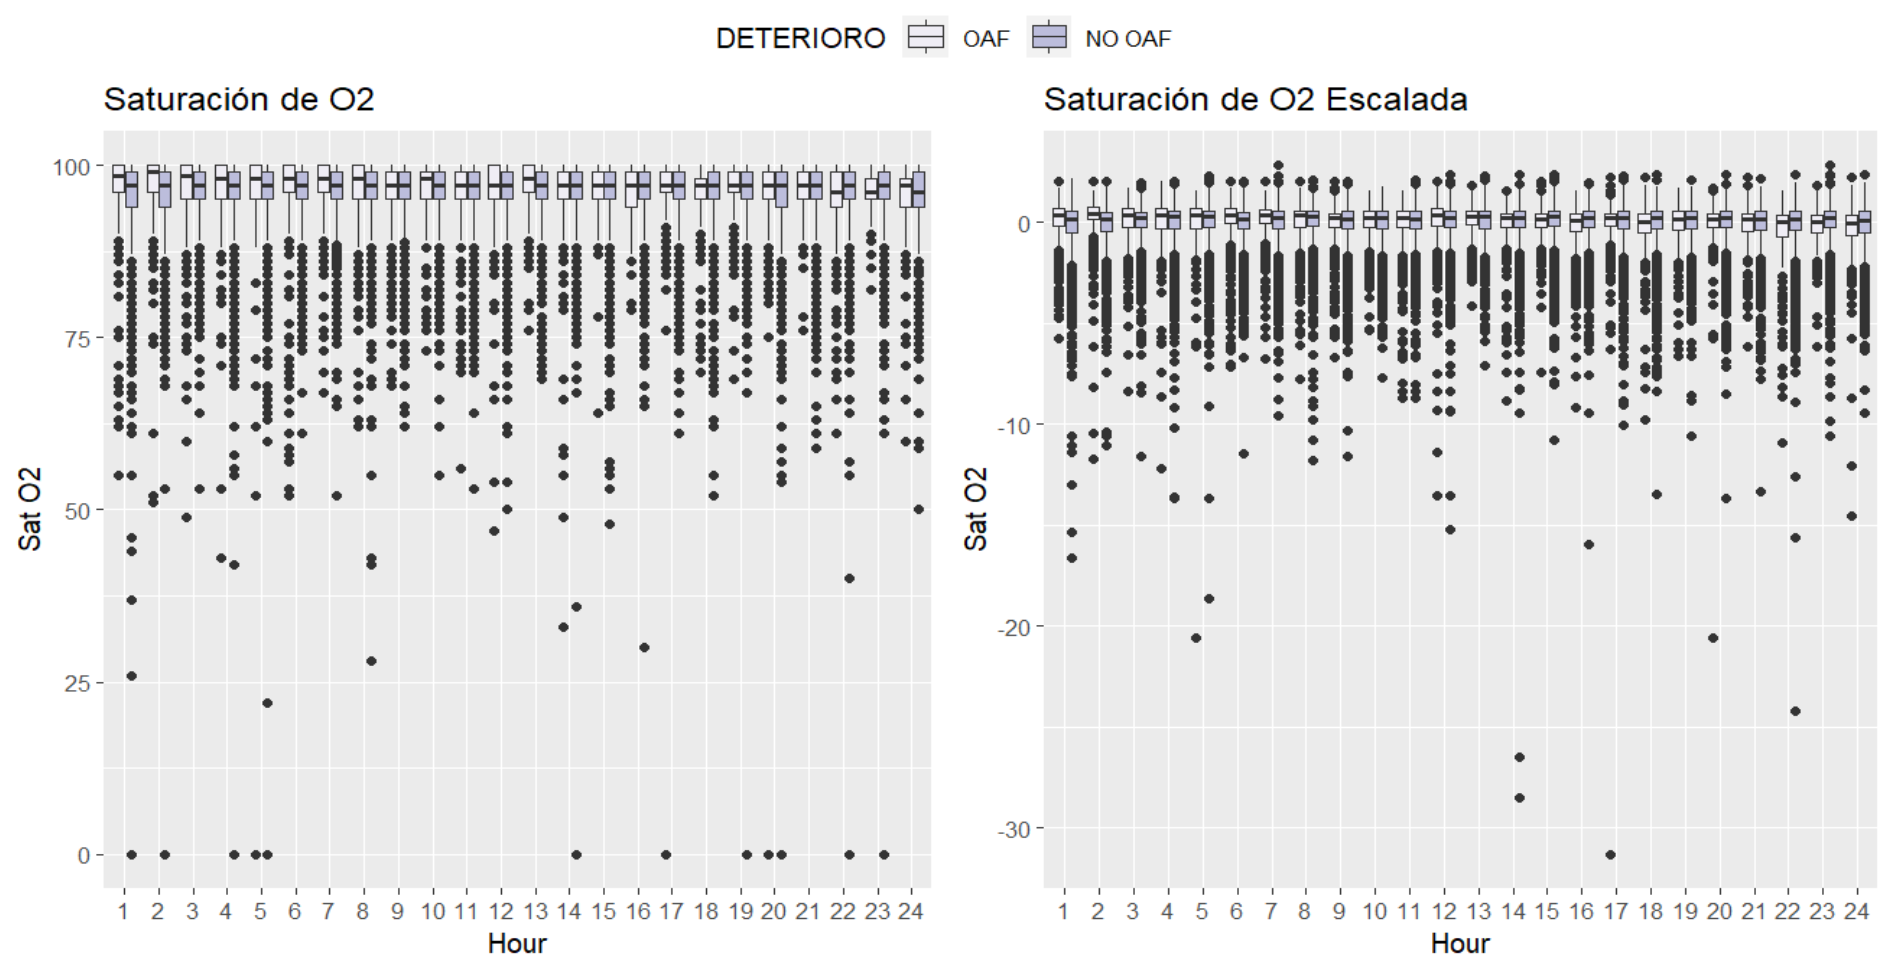
\includegraphics[scale = 0.68]{./img/satO2-boxplot-mean.png}
    \caption{Media Horaria de la \textit{Saturación de Oxígeno} y la \textit{Saturación de Oxígeno Escalada} entre pacientes que sufren DETERIORO y los que no}
    \label{fig:satO2-boxplot-mean}
\end{figure}
\end{landscape}
\restoregeometry